\message{ !name(paper.tex)}%  article.tex (Version 3.3, released 19 January 2008)
%  Article to demonstrate format for SPIE Proceedings
%  Special instructions are included in this file after the
%  symbol %>>>>
%  Numerous commands are commented out, but included to show how
%  to effect various options, e.g., to print page numbers, etc.
%  This LaTeX source file is composed for LaTeX2e.

%  The following commands have been added in the SPIE class 
%  file (spie.cls) and will not be understood in other classes:
%  \supit{}, \authorinfo{}, \skiplinehalf, \keywords{}
%  The bibliography style file is called spiebib.bst, 
%  which replaces the standard style unstr.bst.  

\documentclass[]{spie}  %>>> use for US letter paper
%%\documentclass[a4paper]{spie}  %>>> use this instead for A4 paper
%%\documentclass[nocompress]{spie}  %>>> to avoid compression of citations
%% \addtolength{\voffset}{9mm}   %>>> moves text field down
%% \renewcommand{\baselinestretch}{1.65}   %>>> 1.65 for double spacing, 1.25 for 1.5 spacing 
%  The following command loads a graphics package to include images 
%  in the document. It may be necessary to specify a DVI driver option,
%  e.g., [dvips], but that may be inappropriate for some LaTeX 
%  installations. 
\usepackage{graphicx}
\usepackage{subfig}
\usepackage{amsmath}
\usepackage{amssymb}
\usepackage{hyperref}
\usepackage{float}
\title{Texture mapping 3D planar models of indoor environments with noisy camera poses} 

%>>>> The author is responsible for formatting the 
%  author list and their institutions.  Use  \skiplinehalf 
%  to separate author list from addresses and between each address.
%  The correspondence between each author and his/her address
%  can be indicated with a superscript in italics, 
%  which is easily obtained with \supit{}.

\author{Peter Cheng, Michael Anderson, Stewart He, and Avideh Zakhor
\skiplinehalf
University of California, Berkeley\\
}

 

%%%%%%%%%%%%%%%%%%%%%%%%%%%%%%%%%%%%%%%%%%%%%%%%%%%%%%%%%%%%% 
%>>>> uncomment following for page numbers
% \pagestyle{plain}    
%>>>> uncomment following to start page numbering at 301 
%\setcounter{page}{301} 
 
\begin{document}

\message{ !name(paper.tex) !offset(435) }
\subsection{Image Occlusion}
\label{sec:imageOcclusion}

\begin{figure}
  \centering
  \subfloat[][]{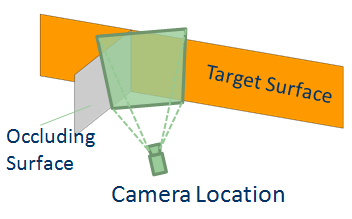
\includegraphics[width=3in]{occlusiondiagram.png}}
   \subfloat[][]{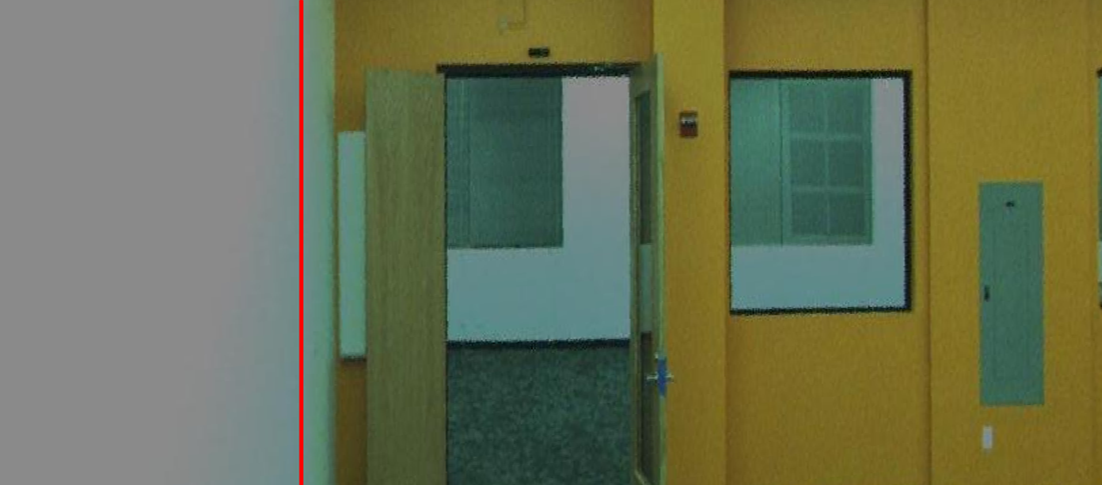
\includegraphics[width=3in,
    height=1.8in]{occlusionimagebad.png}}\\
  \hspace{3in} 
  \subfloat[][]{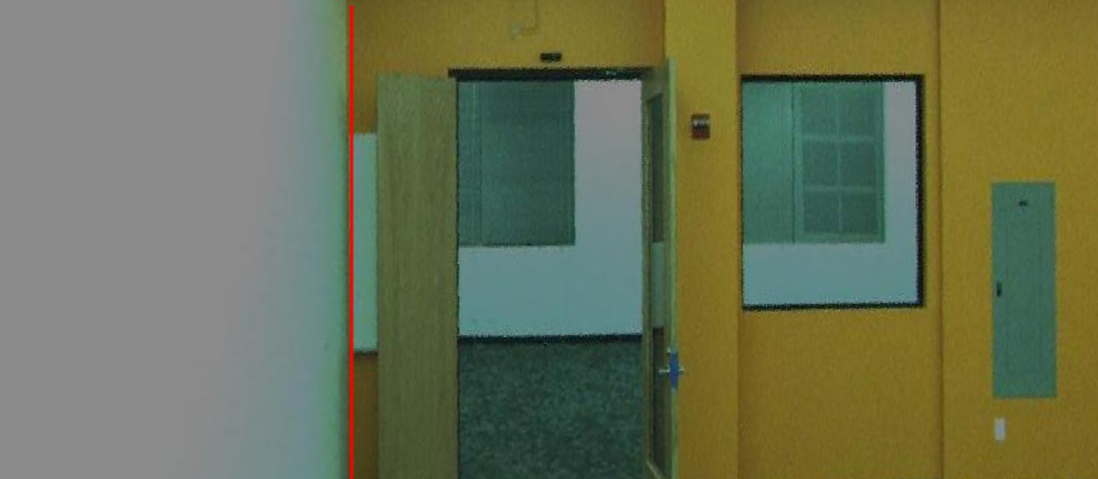
\includegraphics[width=3in,
    height=1.8in]{occlusionimagegood.png}}
  
  \caption{(a) The image from the camera in this diagram contains
    texture that belongs to the grey occluding surface, which should
    not be projected onto the orange target surface; (b) without
    geometry alignment, texture to the left of the red line would be
    removed, which would leave some erroneous texture projected onto
    our target surface; (c) after geometry alignment, the image is
    shifted, resulting in the correct amount of texture being
    removed.}
  \label{fig:occlusion}
\end{figure}

In order to correctly texture surfaces, it is important to detect and
remove parts of image projections containing texture for occluding
surfaces. For instance, in Figure \ref{fig:occlusion}(a), an image
used to texture the orange target surface also contains part of a grey
occluding surface. We remove this incorrect texture by recursively
performing ray-polygon intersection tests between the camera location
and other surfaces \cite{rayintersection}. These intersection tests
are performed at the corners of a grid overlaid upon the target
surface. Where all four corners of a grid section are occluded,
texture is removed. Where one or more corners are occluded, the grid
is subdivided into four, and the process repeats. Occlusion checking
works entirely with geometry, so by ensuring that images match
geometry using \ref{sec:geometryAlignment}'s alignment procedure,
texture belonging to other surfaces is accurately removed, as seen in
Figure \ref{fig:occlusion}(b).

\message{ !name(paper.tex) !offset(852) }

\end{document} 
